\documentclass[varwidth]{standalone}

\usepackage{tikz}
\usetikzlibrary{shapes.geometric, arrows, calc, positioning}

\tikzstyle{morning} = [rectangle, rounded corners, minimum width=3cm, minimum
height=2cm,text centered, text width = 3cm, draw=black, fill=green!30]

\tikzstyle{afternoon} = [rectangle, rounded corners, minimum width=3cm, minimum
height=2cm,text centered, text width = 3cm, draw=black, fill=red!30]

\tikzstyle{evening} = [rectangle, rounded corners, minimum width=3cm, minimum
height=2cm,text centered, text width = 3cm, draw=black, fill=blue!30]


\tikzstyle{arrow} = [thick,->,>=stealth]



\title{Timetable}
\author{Qiyuan Pu}

\begin{document}
\maketitle{}
\begin{figure}
  \centering

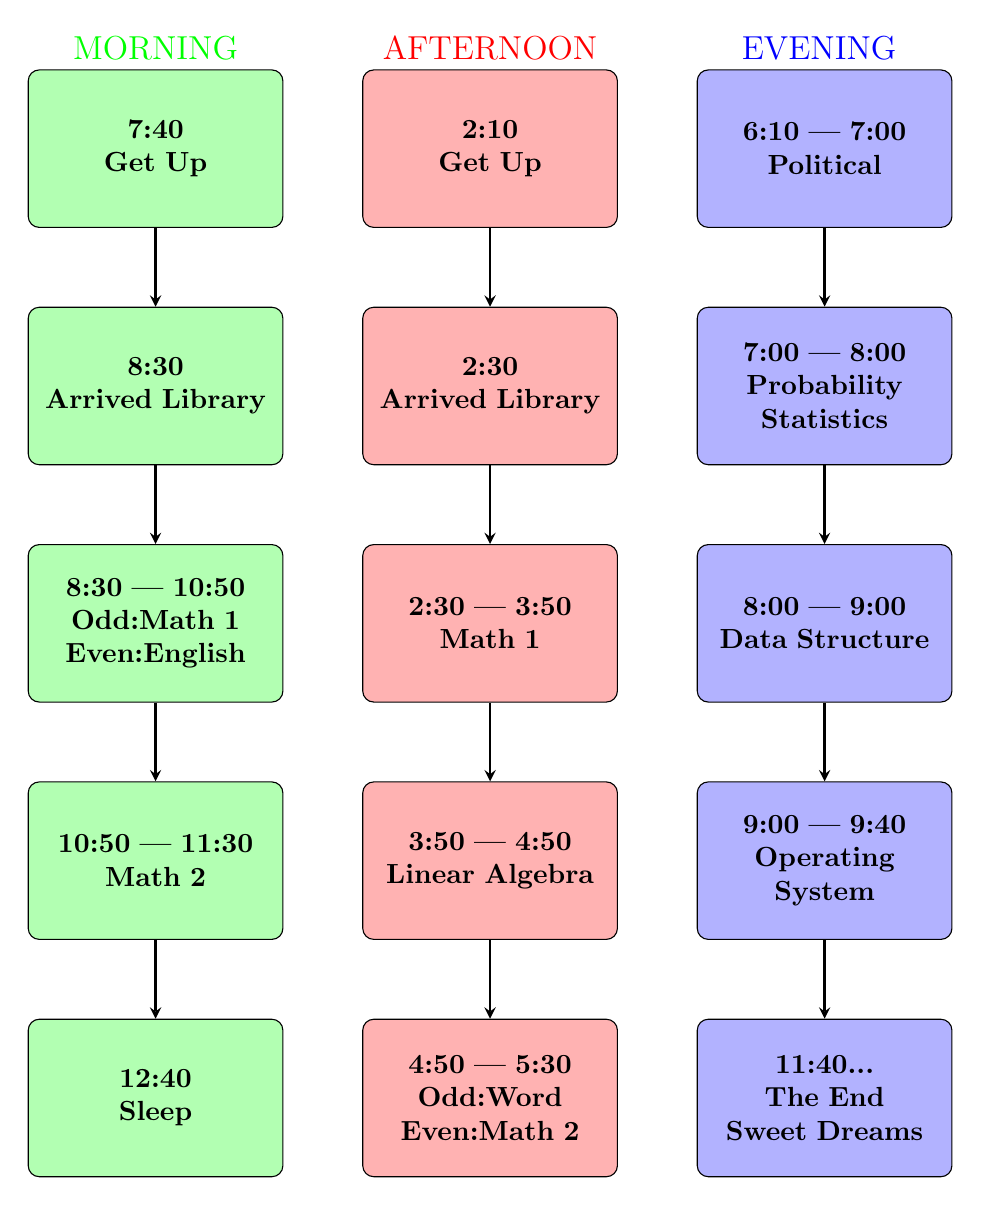
\begin{tikzpicture}
  \node (mor2) [morning, label=above: {\large \color{green} MORNING}] {\bf 7:40 \\ Get Up};
  \node (mor3) [morning, below=of mor2] {\bf 8:30 \\ Arrived Library};
  \node (mor4) [morning, below=of mor3] {\bf 8:30 — 10:50 Odd:Math 1 Even:English};
  \node (mor5) [morning, below=of mor4] {\bf 10:50 — 11:30 \\ Math 2};
  \node (mor6) [morning, below=of mor5] {\bf 12:40 \\ Sleep};

  \node (aft2) [afternoon, right=of mor2, label=above: {\large \color{red} AFTERNOON}] {\bf 2:10 \\ Get Up};
  \node (aft3) [afternoon, below=of aft2] {\bf 2:30 \\ Arrived Library};
  \node (aft4) [afternoon, below=of aft3] {\bf 2:30 — 3:50 \\ Math 1};
  \node (aft5) [afternoon, below=of aft4] {\bf 3:50 — 4:50 \\ Linear Algebra};
  \node (aft6) [afternoon, below=of aft5] {\bf 4:50 — 5:30 \\ Odd:Word Even:Math 2};

  \node (eve1) [evening, right=of aft2, label=above: {\large \color{blue} EVENING }] {\bf 6:10 — 7:00 \\ Political};
  \node (eve2) [evening, below=of eve1] {\bf 7:00 — 8:00 \\ Probability Statistics};
  \node (eve3) [evening, below=of eve2] {\bf 8:00 — 9:00 \\ Data Structure};
  \node (eve4) [evening, below=of eve3] {\bf 9:00 — 9:40 \\ Operating System};
  \node (eve5) [evening, below=of eve4] {\bf 11:40... \\ The End \\ Sweet Dreams};

  \draw [arrow] (eve4) -- (eve5);
  \draw [arrow] (eve3) -- (eve4);
  \draw [arrow] (eve2) -- (eve3);
  \draw [arrow] (eve1) -- (eve2);
  \draw [arrow] (mor3) -- (mor4);
  \draw [arrow] (mor4) -- (mor5);
  \draw [arrow] (mor5) -- (mor6);
  \draw [arrow] (mor2) -- (mor3);
  \draw [arrow] (aft2) -- (aft3);
  \draw [arrow] (aft3) -- (aft4);
  \draw [arrow] (aft4) -- (aft5);
  \draw [arrow] (aft5) -- (aft6);
\end{tikzpicture}

\textcolor{red}{Fighting}

\end{figure}


\end{document}



%%% Local Variables:
%%% mode: latex
%%% TeX-master: t
%%% End:
